System:
\begin{equation}
	a(\vec x(t), u(t), t) = 
	\begin{bmatrix}
		\dot x_1(t) \\
		\dot x_2(t)
	\end{bmatrix}
= 
	\begin{bmatrix}
	-x_1(t) + u(t) \\
	-x_2(t) + u(t)
	\end{bmatrix}
\end{equation}
\begin{equation}
	\vec{x}(t) = 
	\begin{bmatrix}
		-1 &  0 \\
		 0 & -1
	\end{bmatrix}
\vec{x}(t)+
\begin{bmatrix}
		1 \\
		1
	\end{bmatrix}u
\end{equation}
For minimum time:
$$J = t_f - t_0 = \int_{t_0}^{t_f} dt$$
Hamiltonian matrix:
$$\mathcal{H} =  g(\vec x(t), u(t), t) + {\vec{p}(t)}^Ta(\vec x(t), u(t), t)$$
$$\mathcal{H} = 1 + \begin{bmatrix} 
	p_1(t) & p_2(t)
\end{bmatrix} 	\begin{bmatrix}
-x_1(t) + u(t) \\
-x_2(t) + u(t)
\end{bmatrix}$$
\begin{equation}\label{HamiltonianQ4}
	\mathcal{H} = 1 - p_21(t)x_1(t) + p_1(t)u(t) - p_2(t)x_2(t) +p_2(t)u(t) 
\end{equation}
Euler–Lagrange equation:
\begin{align}
	\dot{\vec{x}} &= \dfrac{\partial \mathcal{H} }{\partial \vec{p}} = a(\vec x(t), u(t), t)\\
	\dot{\vec{p}} &= -\dfrac{\partial \mathcal{H} }{\partial \vec{x}} \\
	{\vec{0}} &= \dfrac{\partial \mathcal{H} }{\partial \vec{u}}
\end{align}
Now  we use equation \ref{HamiltonianQ4} to solve Euler-Lagrange equation.
\begin{equation}\label{diffpQ4}
	\begin{bmatrix}
		\dot{p_1}\\
		\dot{p_2}\\
	\end{bmatrix} = \begin{bmatrix}
		-\dfrac{\partial \mathcal{H}}{\partial x_1} \\[10 pt]
		-\dfrac{\partial \mathcal{H}}{\partial x_2}
	\end{bmatrix} = \begin{bmatrix}
	p_1\\
	p_2
	\end{bmatrix}
\end{equation} 
Answer of equation \ref{diffpQ4} is:
\begin{equation}\label{SolvepQ4}
	\begin{bmatrix}
		p_1(t)\\
		p_2(t)
	\end{bmatrix} = \begin{bmatrix}
	C_1\exp(-t)\\
	C_2\exp(-t)
	\end{bmatrix} 
\end{equation}
From Euler-Lagrange equation:
\begin{equation}\label{AnsUQ4}
	{\vec{0}} = \dfrac{\partial \mathcal{H} }{\partial \vec{u}} \to 
	p_4\cos(u) = p_1 + p_2 = \left(  C_1 + C_2  \right)\exp(-t)
\end{equation}
From equation \ref{AnsUQ4} we can find out sign of $\dfrac{\partial \mathcal{H} }{\partial \vec{u}}$ is the same for all time so there is no switch. So for all time $u(t)$ is constant and it may be $1$ or $-1$ for all time. Now we simulate system with this $u(t)$.
\begin{equation}
	a(\vec x(t), u(t), t) = 
	\begin{bmatrix}
		\dot x_1(t) \\
		\dot x_2(t)
	\end{bmatrix}
	= 
	\begin{bmatrix}
		-x_1(t) \pm 1 \\
		-x_2(t)  \pm 1
	\end{bmatrix}
\end{equation}
Differential equation answers:
\begin{equation}
	\begin{bmatrix}
		x_1(t) \\
		x_2(t)
	\end{bmatrix}
	= 
	\begin{bmatrix}
		C_3\exp(-t) \pm 1 \\
		C_4\exp(-t)  \pm 1
	\end{bmatrix}
\end{equation}
\begin{itemize}
	%%%%%%%%%%%%%%%% u = 1 %%%%%%%%%%%%%%%% 
	\item $u(t) = 1$
	\begin{equation}\label{ansxu1Q4}
		\begin{bmatrix}
			x_1(t) \\
			x_2(t)
		\end{bmatrix}
		= 
		\begin{bmatrix}
			C_3\exp(-t) + 1 \\
			C_4\exp(-t) + 1
		\end{bmatrix}
	\end{equation}
From equation \ref{ansxu1Q4}:
$$x_1(t) = C_3\exp(-t) + 1 \to \exp(-t) = \dfrac{x_1(t)-1}{C_3}\xrightarrow{x_2(t)=C_4\exp(-t) + 1} x_2(t) = \dfrac{C_4}{C_3}x_1(t) -\dfrac{C_4}{C_3} +1$$
Assume $\dfrac{C_4}{C_3} = C_5$:
$$x_2(t) = C_5x_1(t)-C_5 +1$$
\begin{figure}[H]
	\caption{$u(t) = 1$, $x_1$ and $x_2$ for different $C_5$}\label{x1x2u1Q4}
	\centering
	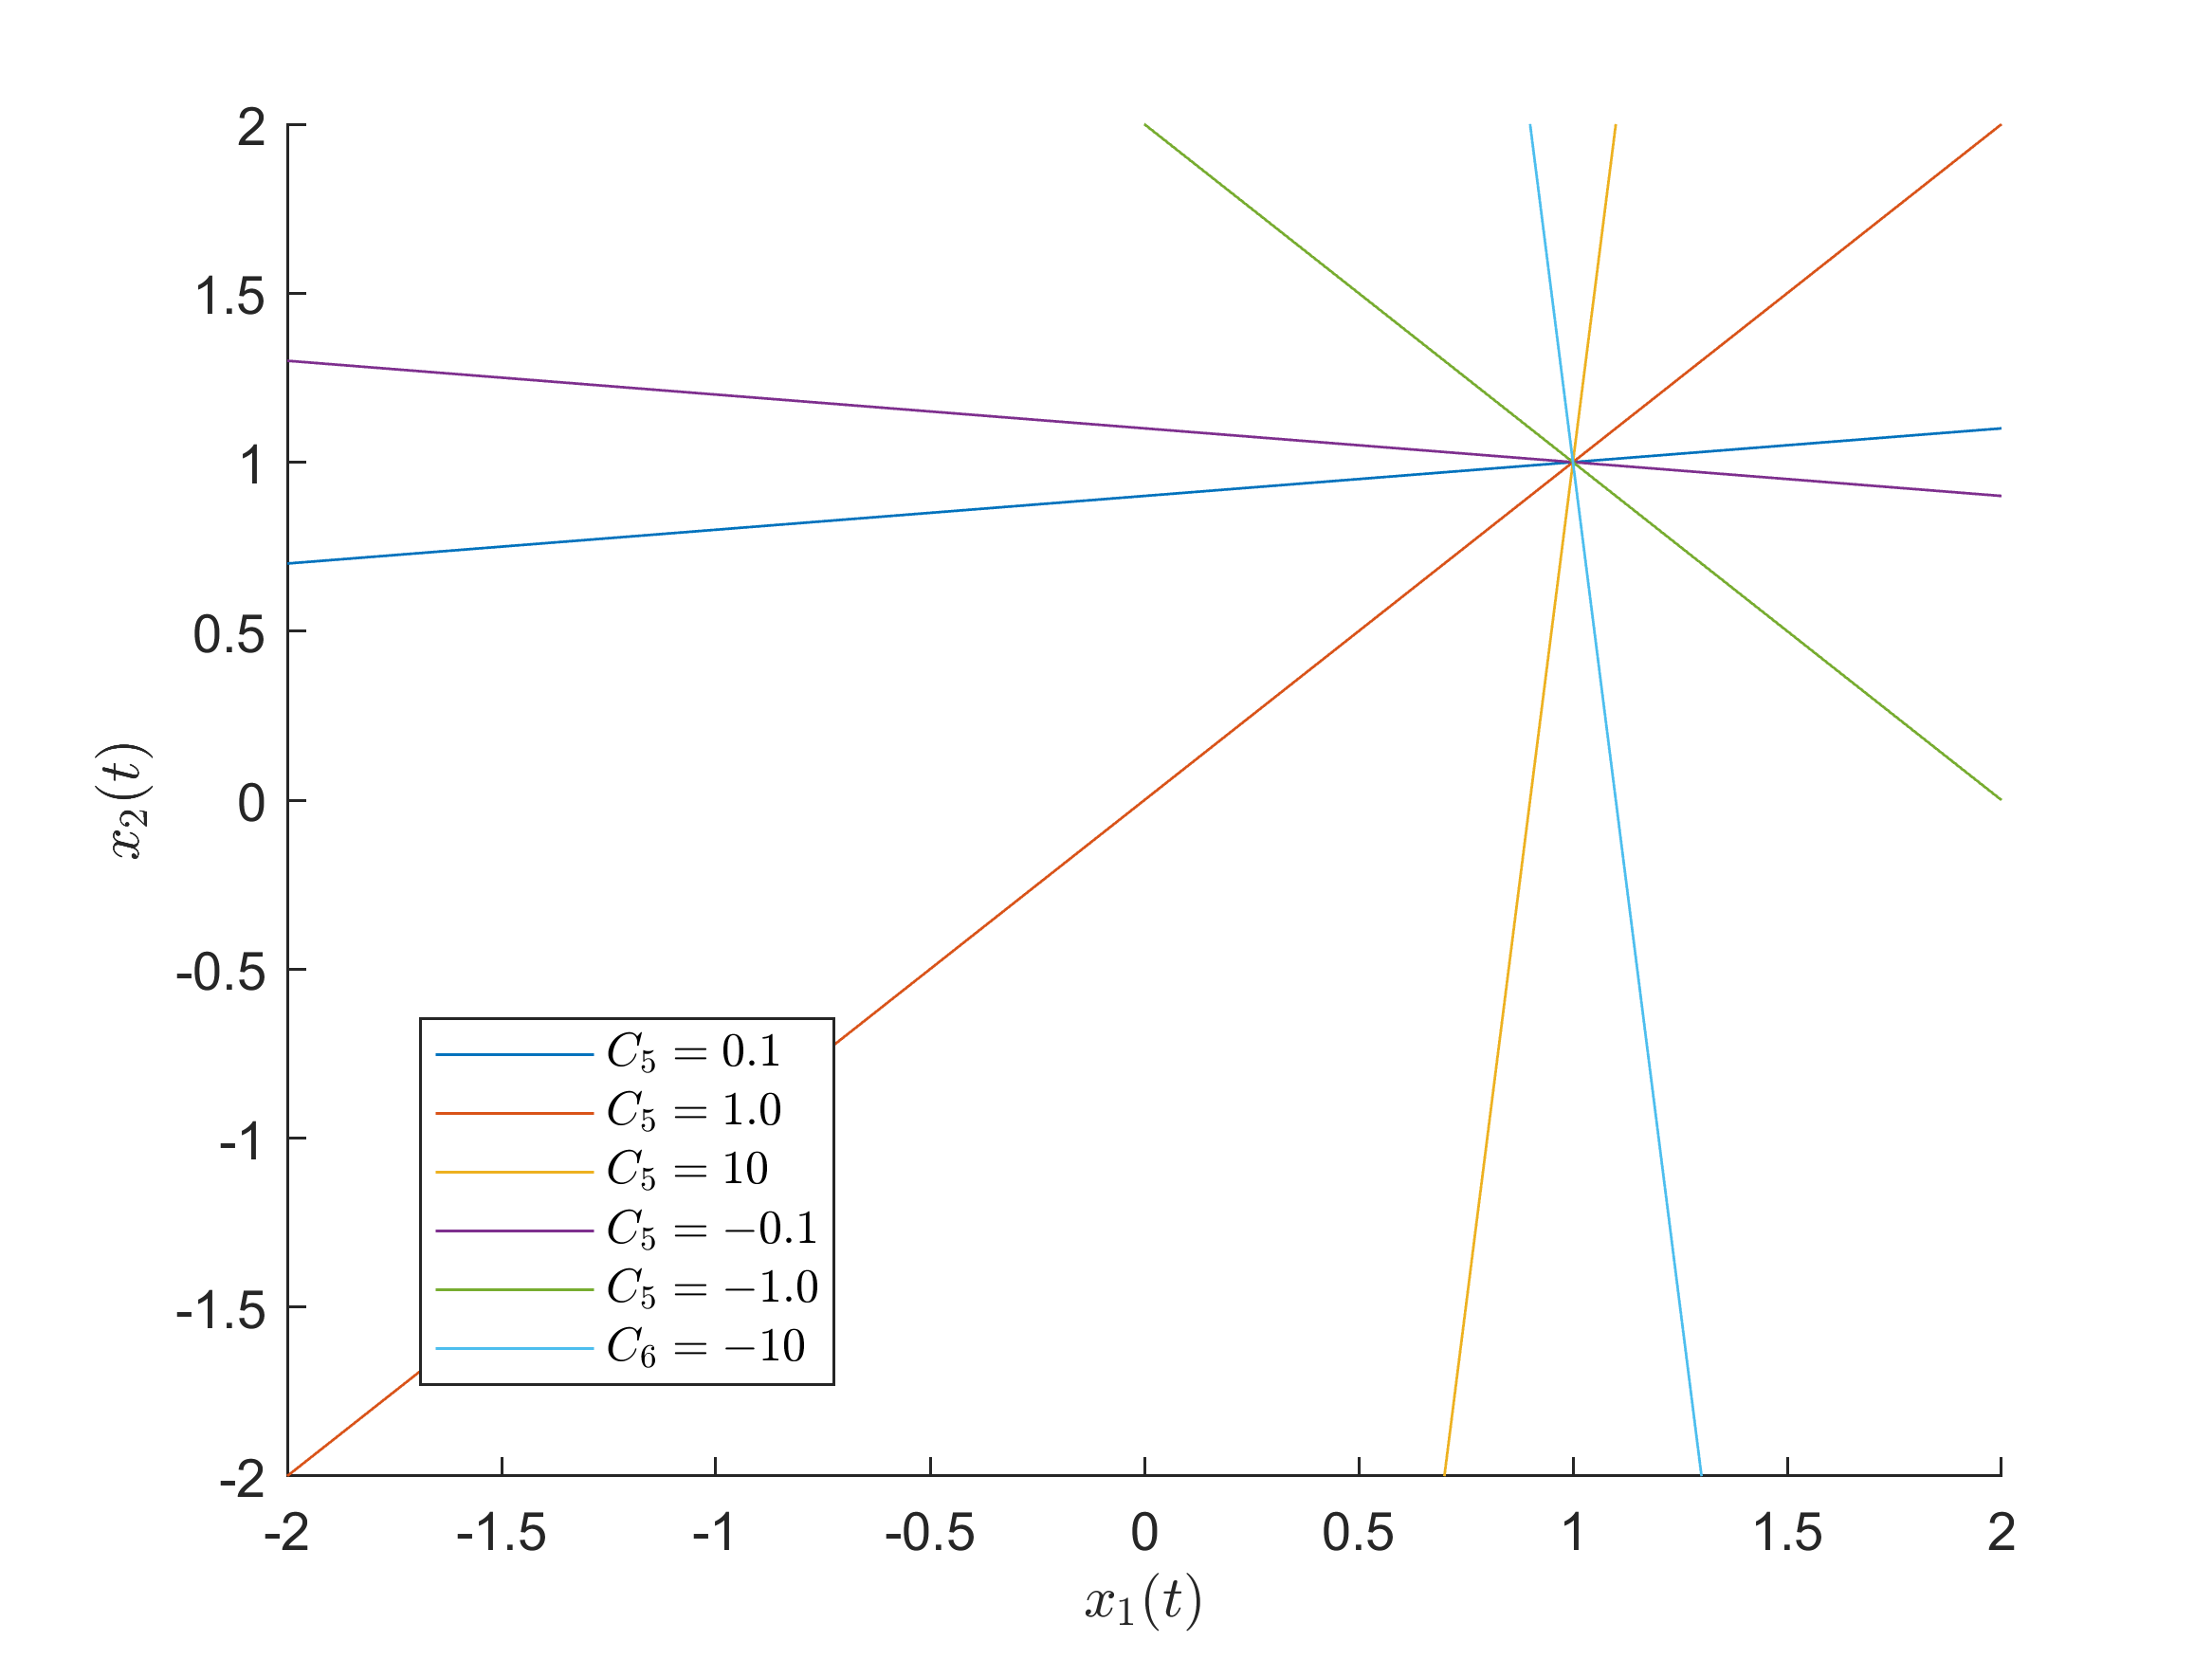
\includegraphics[width=12cm]{../Code/Q4/figures/lowu1x1x2mod.png}
\end{figure}
From figure \ref{x1x2u1Q4} we can know that every point goes to $\begin{bmatrix}
	1\\1
\end{bmatrix}$ and this is direction of function in time. From figure \ref{x1x2u1Q4} we can know that switch curve is $x_1 = x_2$.
\begin{figure}[H]
	\caption{switch curve in $u(t) = 1$}\label{x1x2u1Q4SC}
	\centering
	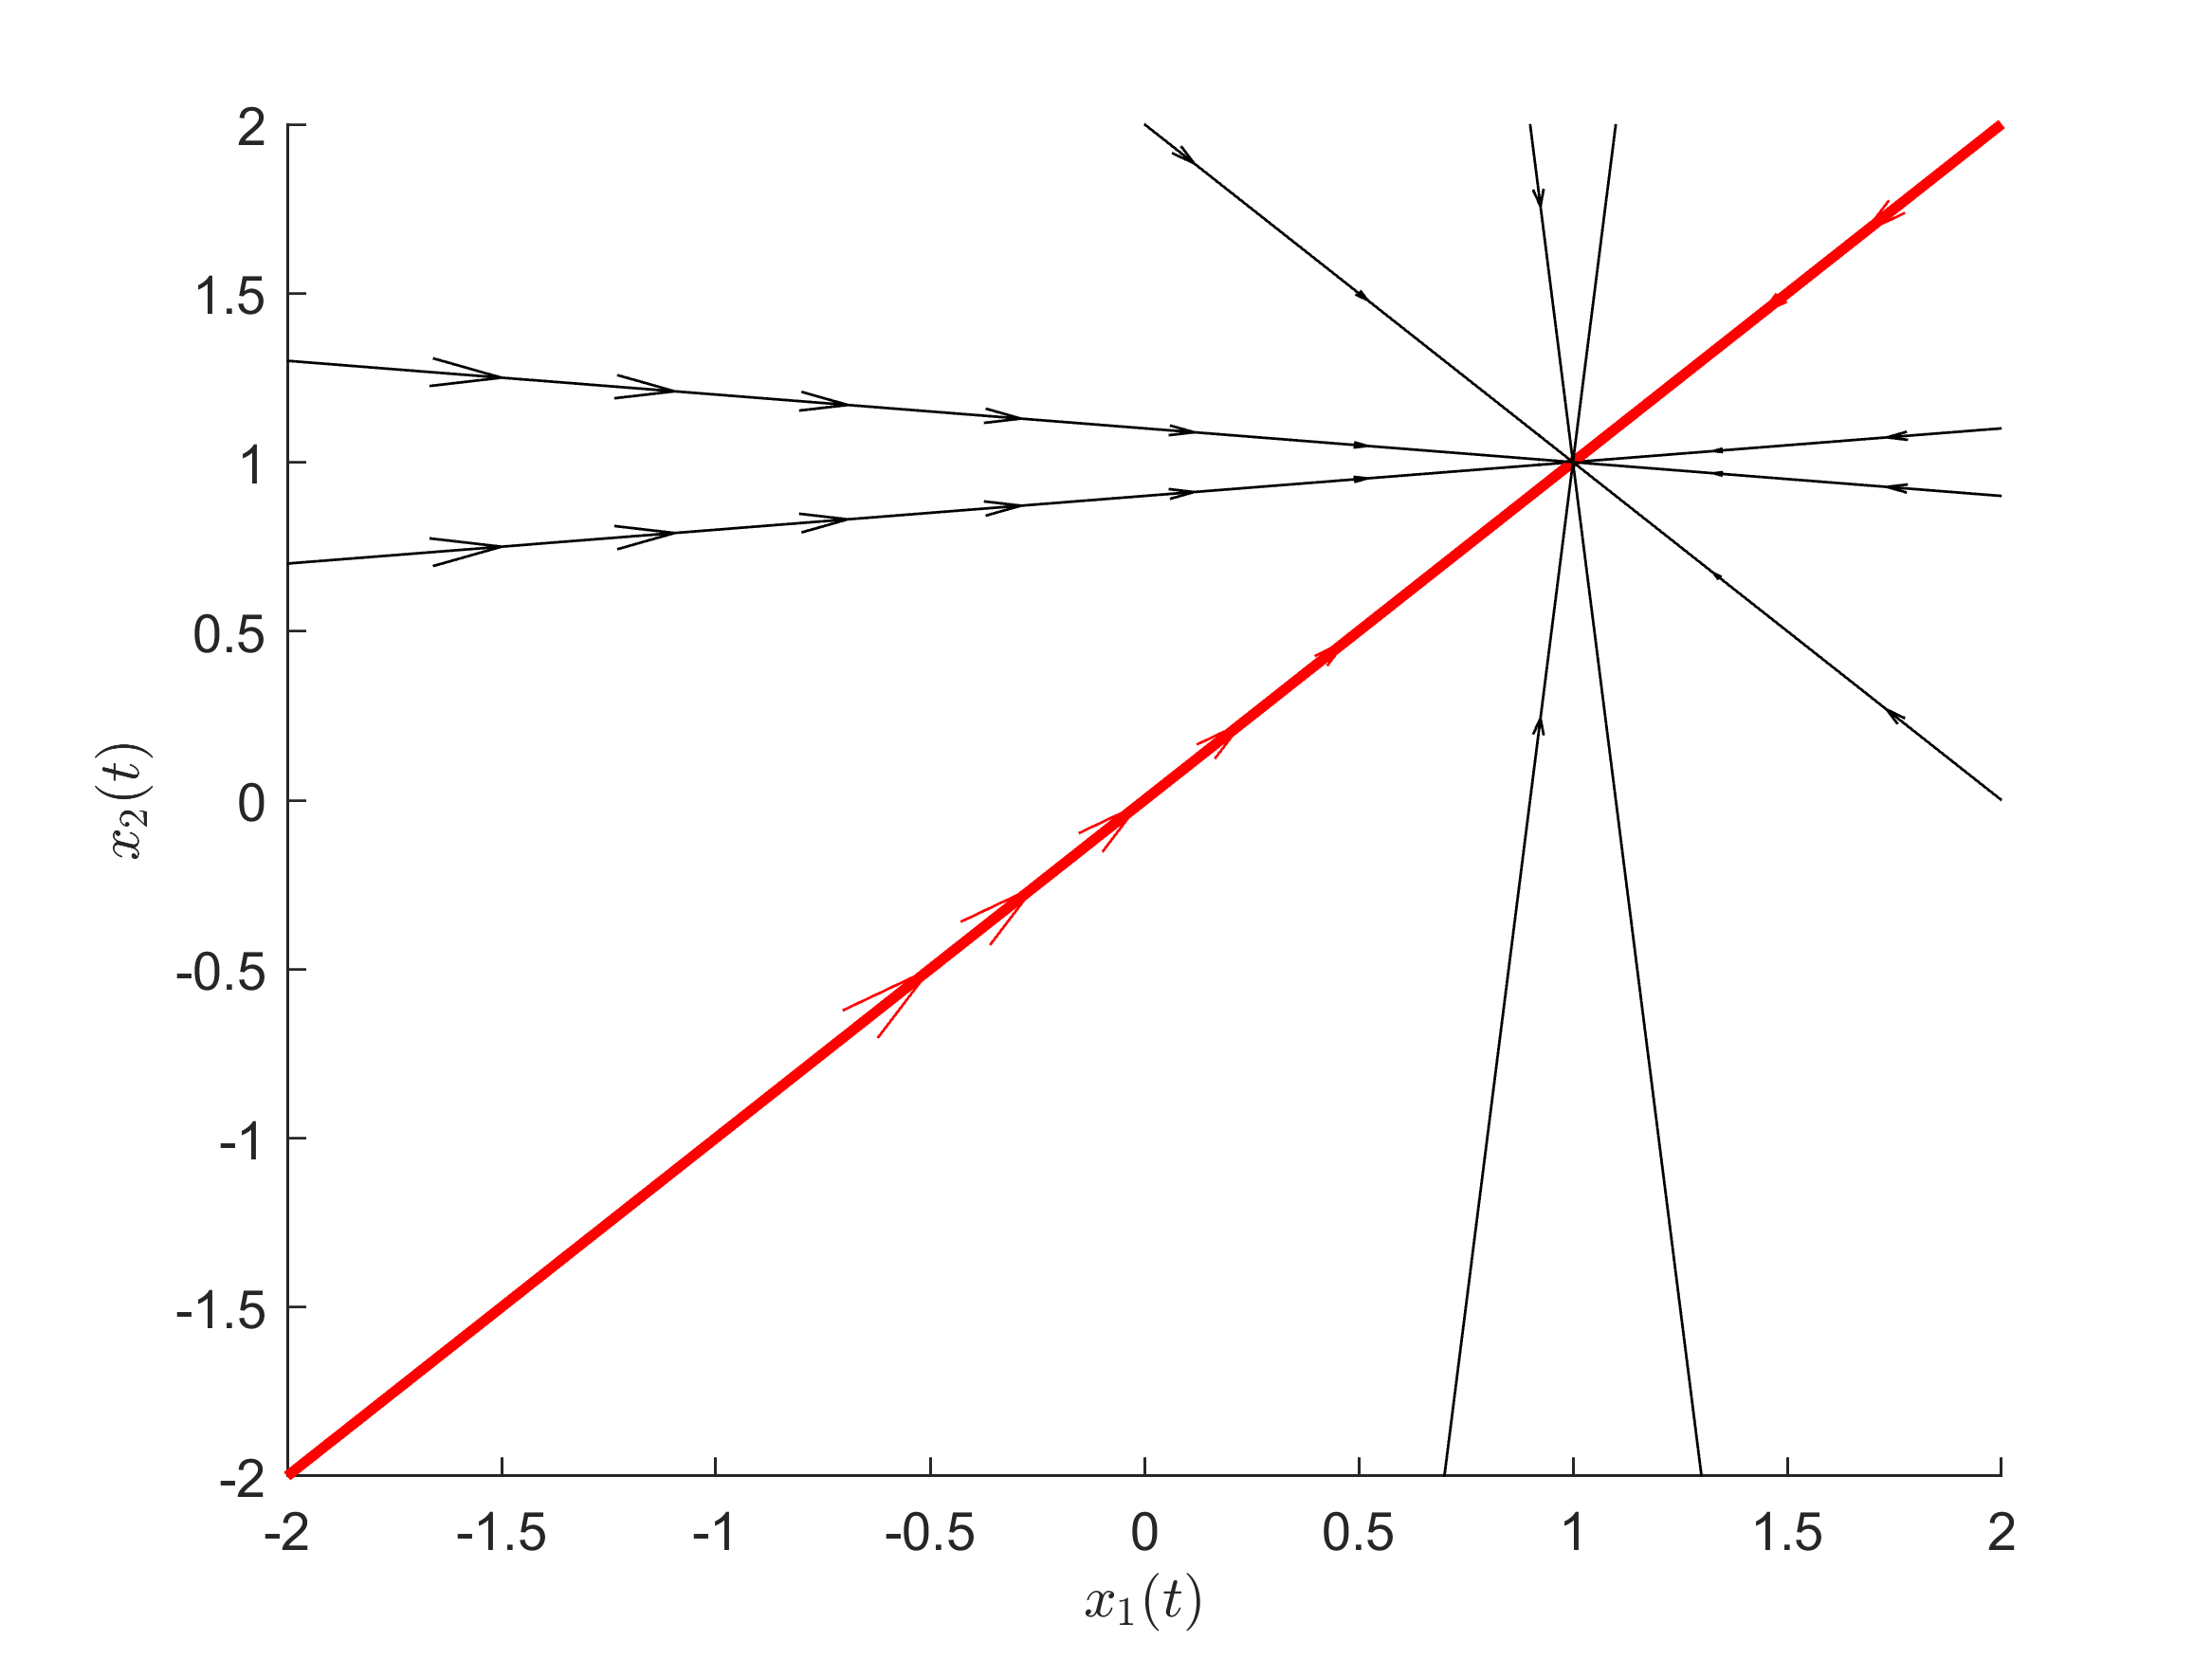
\includegraphics[width=12cm]{../Code/Q4/figures/lowu1x1x2SC.png}
\end{figure}
In figure \ref{x1x2u1Q4SC} you can see switch curve(red line).
	%%%%%%%%%%%%%%%% u = -1 %%%%%%%%%%%%%%%% 
\item $u(t) = -1$
\begin{equation}\label{ansxu-1Q4}
	\begin{bmatrix}
		x_1(t) \\
		x_2(t)
	\end{bmatrix}
	= 
	\begin{bmatrix}
		C_3\exp(-t) - 1 \\
		C_4\exp(-t) - 1
	\end{bmatrix}
\end{equation}
From equation \ref{ansxu-1Q4}:
$$x_1(t) = C_3\exp(-t) - 1 \to \exp(-t) = \dfrac{x_1(t)+1}{C_3}\xrightarrow{x_2(t)=C_4\exp(-t) - 1} x_2(t) = \dfrac{C_4}{C_3}x_1(t)+\dfrac{C_4}{C_3}-1$$
Assume $\dfrac{C_4}{C_3} = C_5$:
$$x_2(t) =C_5x_1(t)+C_5 -1$$
\begin{figure}[H]
	\caption{$u(t) = -1$, $x_1$ and $x_2$ for different $C_5$}\label{x1x2u-1Q4}
	\centering
	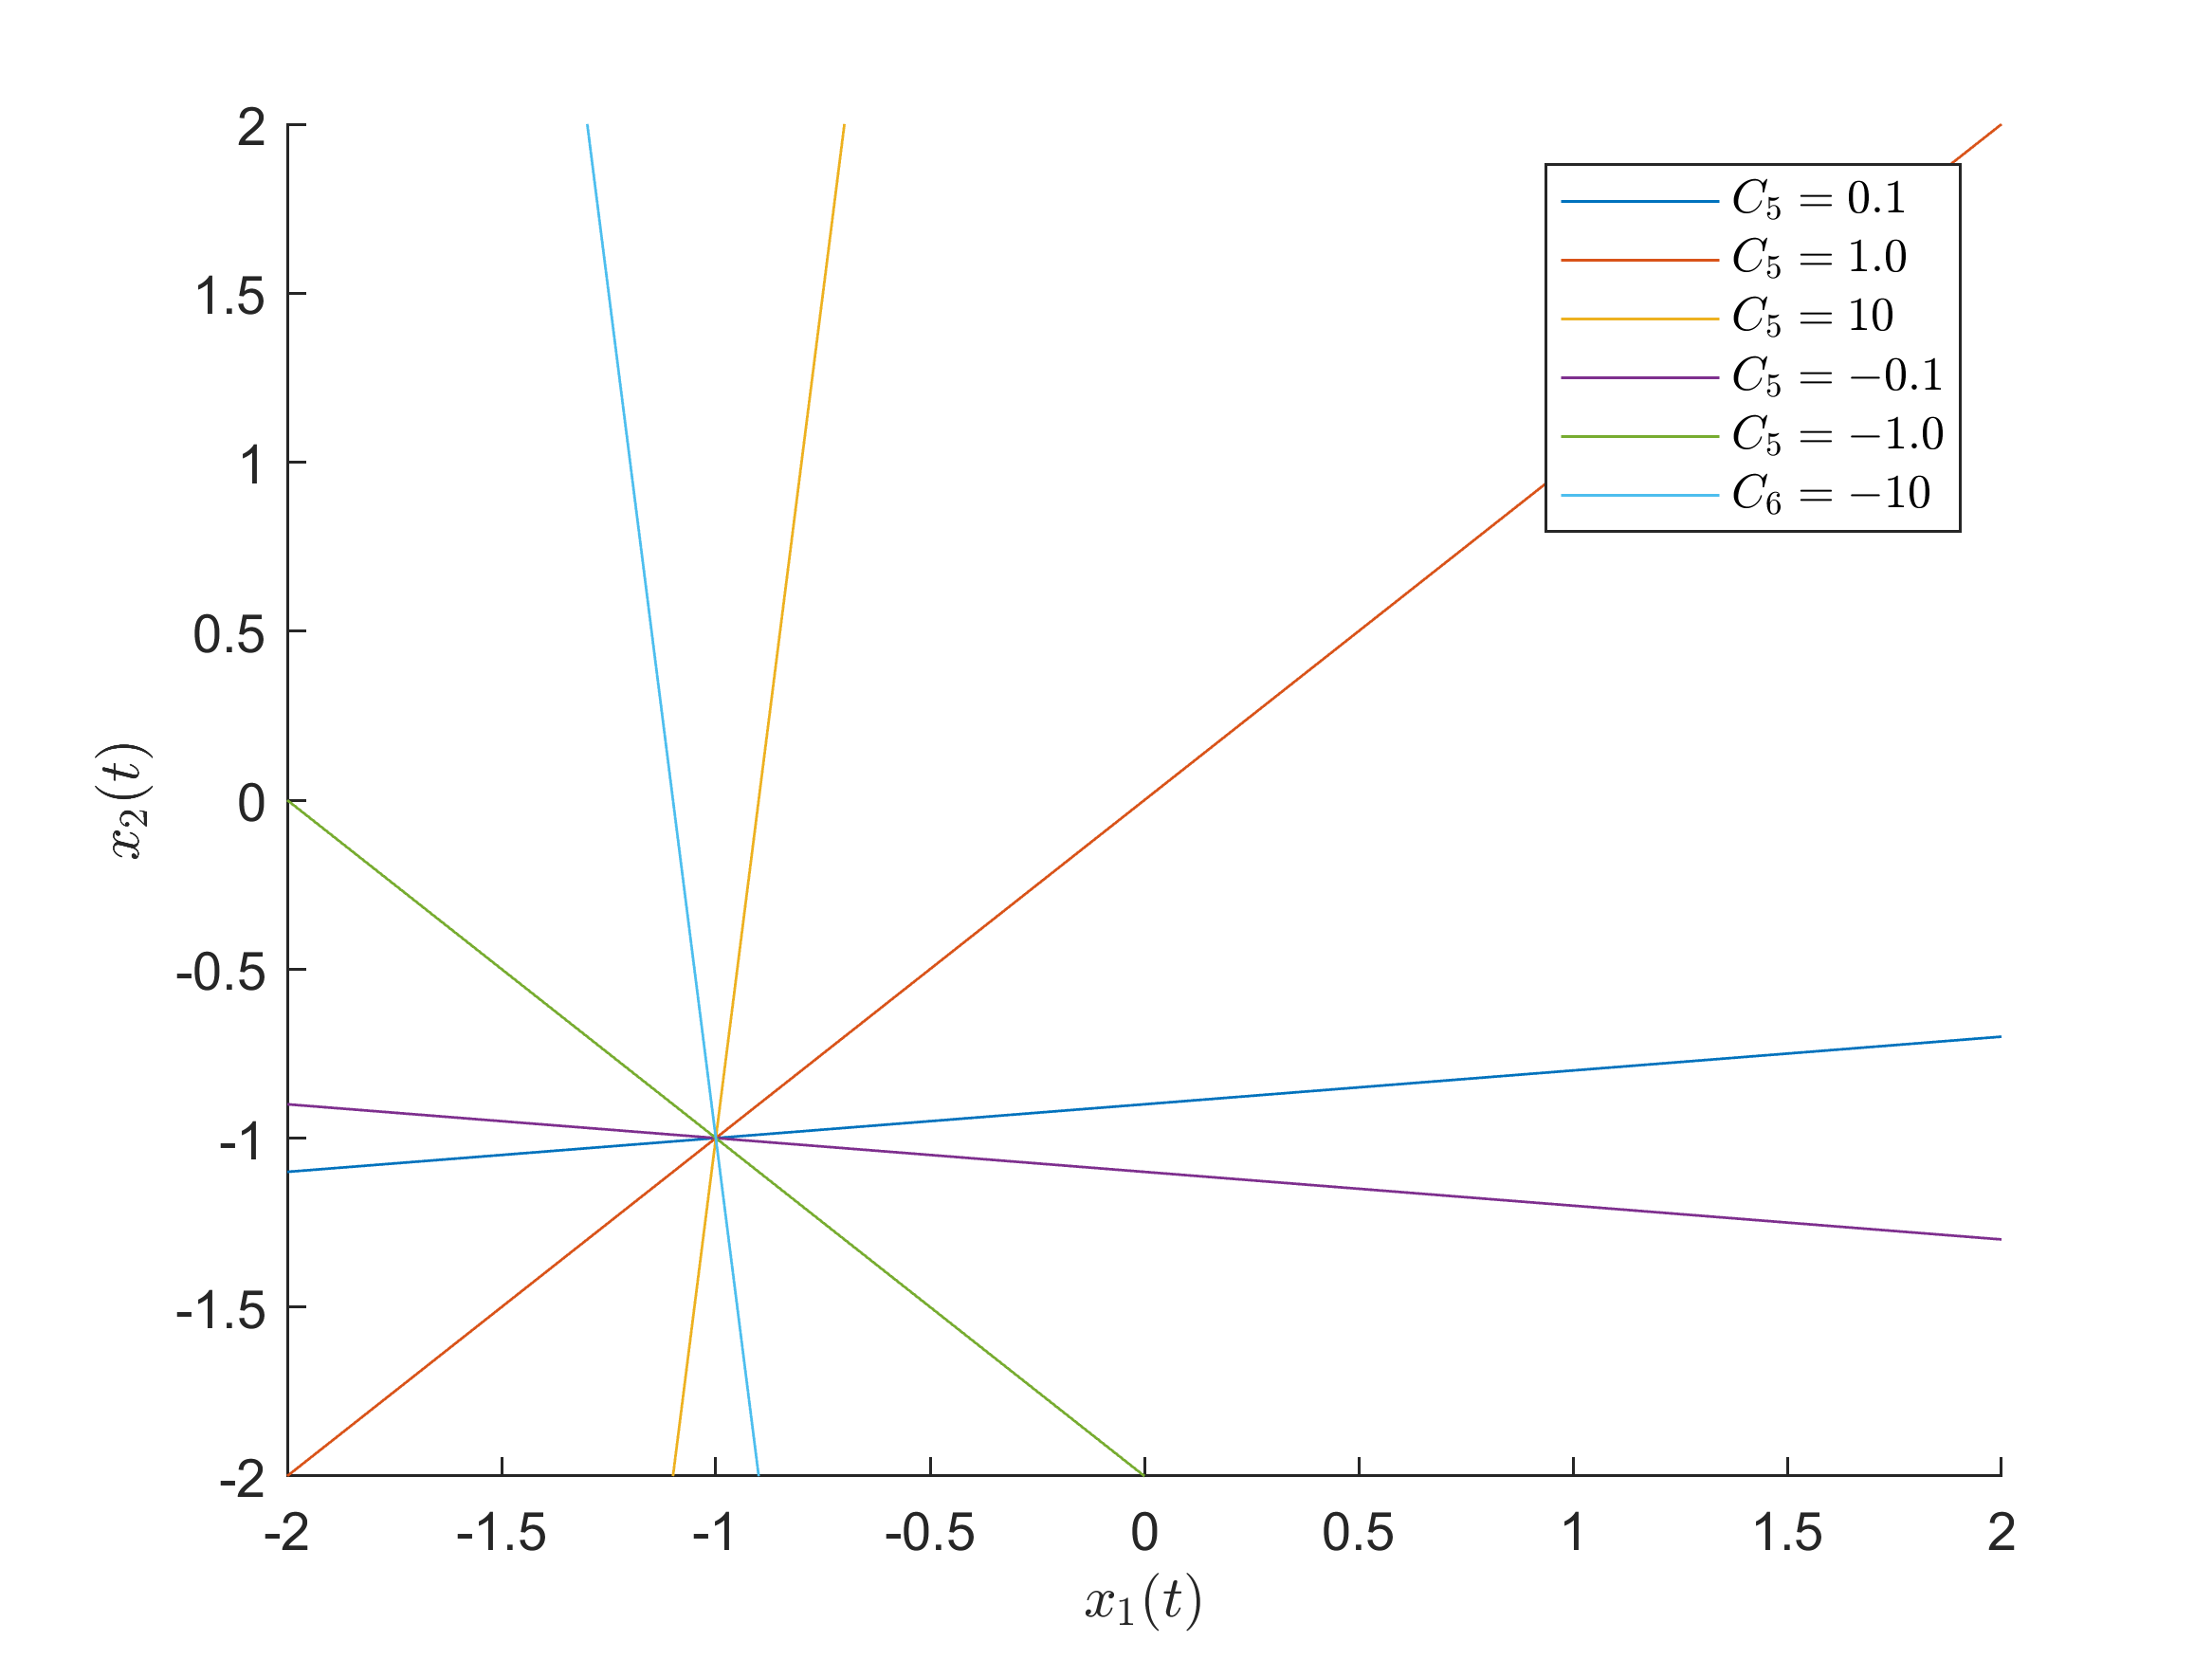
\includegraphics[width=12cm]{../Code/Q4/figures/lowum1x1x2.png}
\end{figure}
From figure \ref{x1x2u-1Q4} we can know that every point goes to $\begin{bmatrix}
	-1\\-1
\end{bmatrix}$ and this is direction of function in time. From figure \ref{x1x2u-1Q4} we can know that switch curve is $x_1 = x_2$.
\begin{figure}[H]
	\caption{switch curve in $u(t) = -1$}\label{x1x2u-1Q4SC}
	\centering
	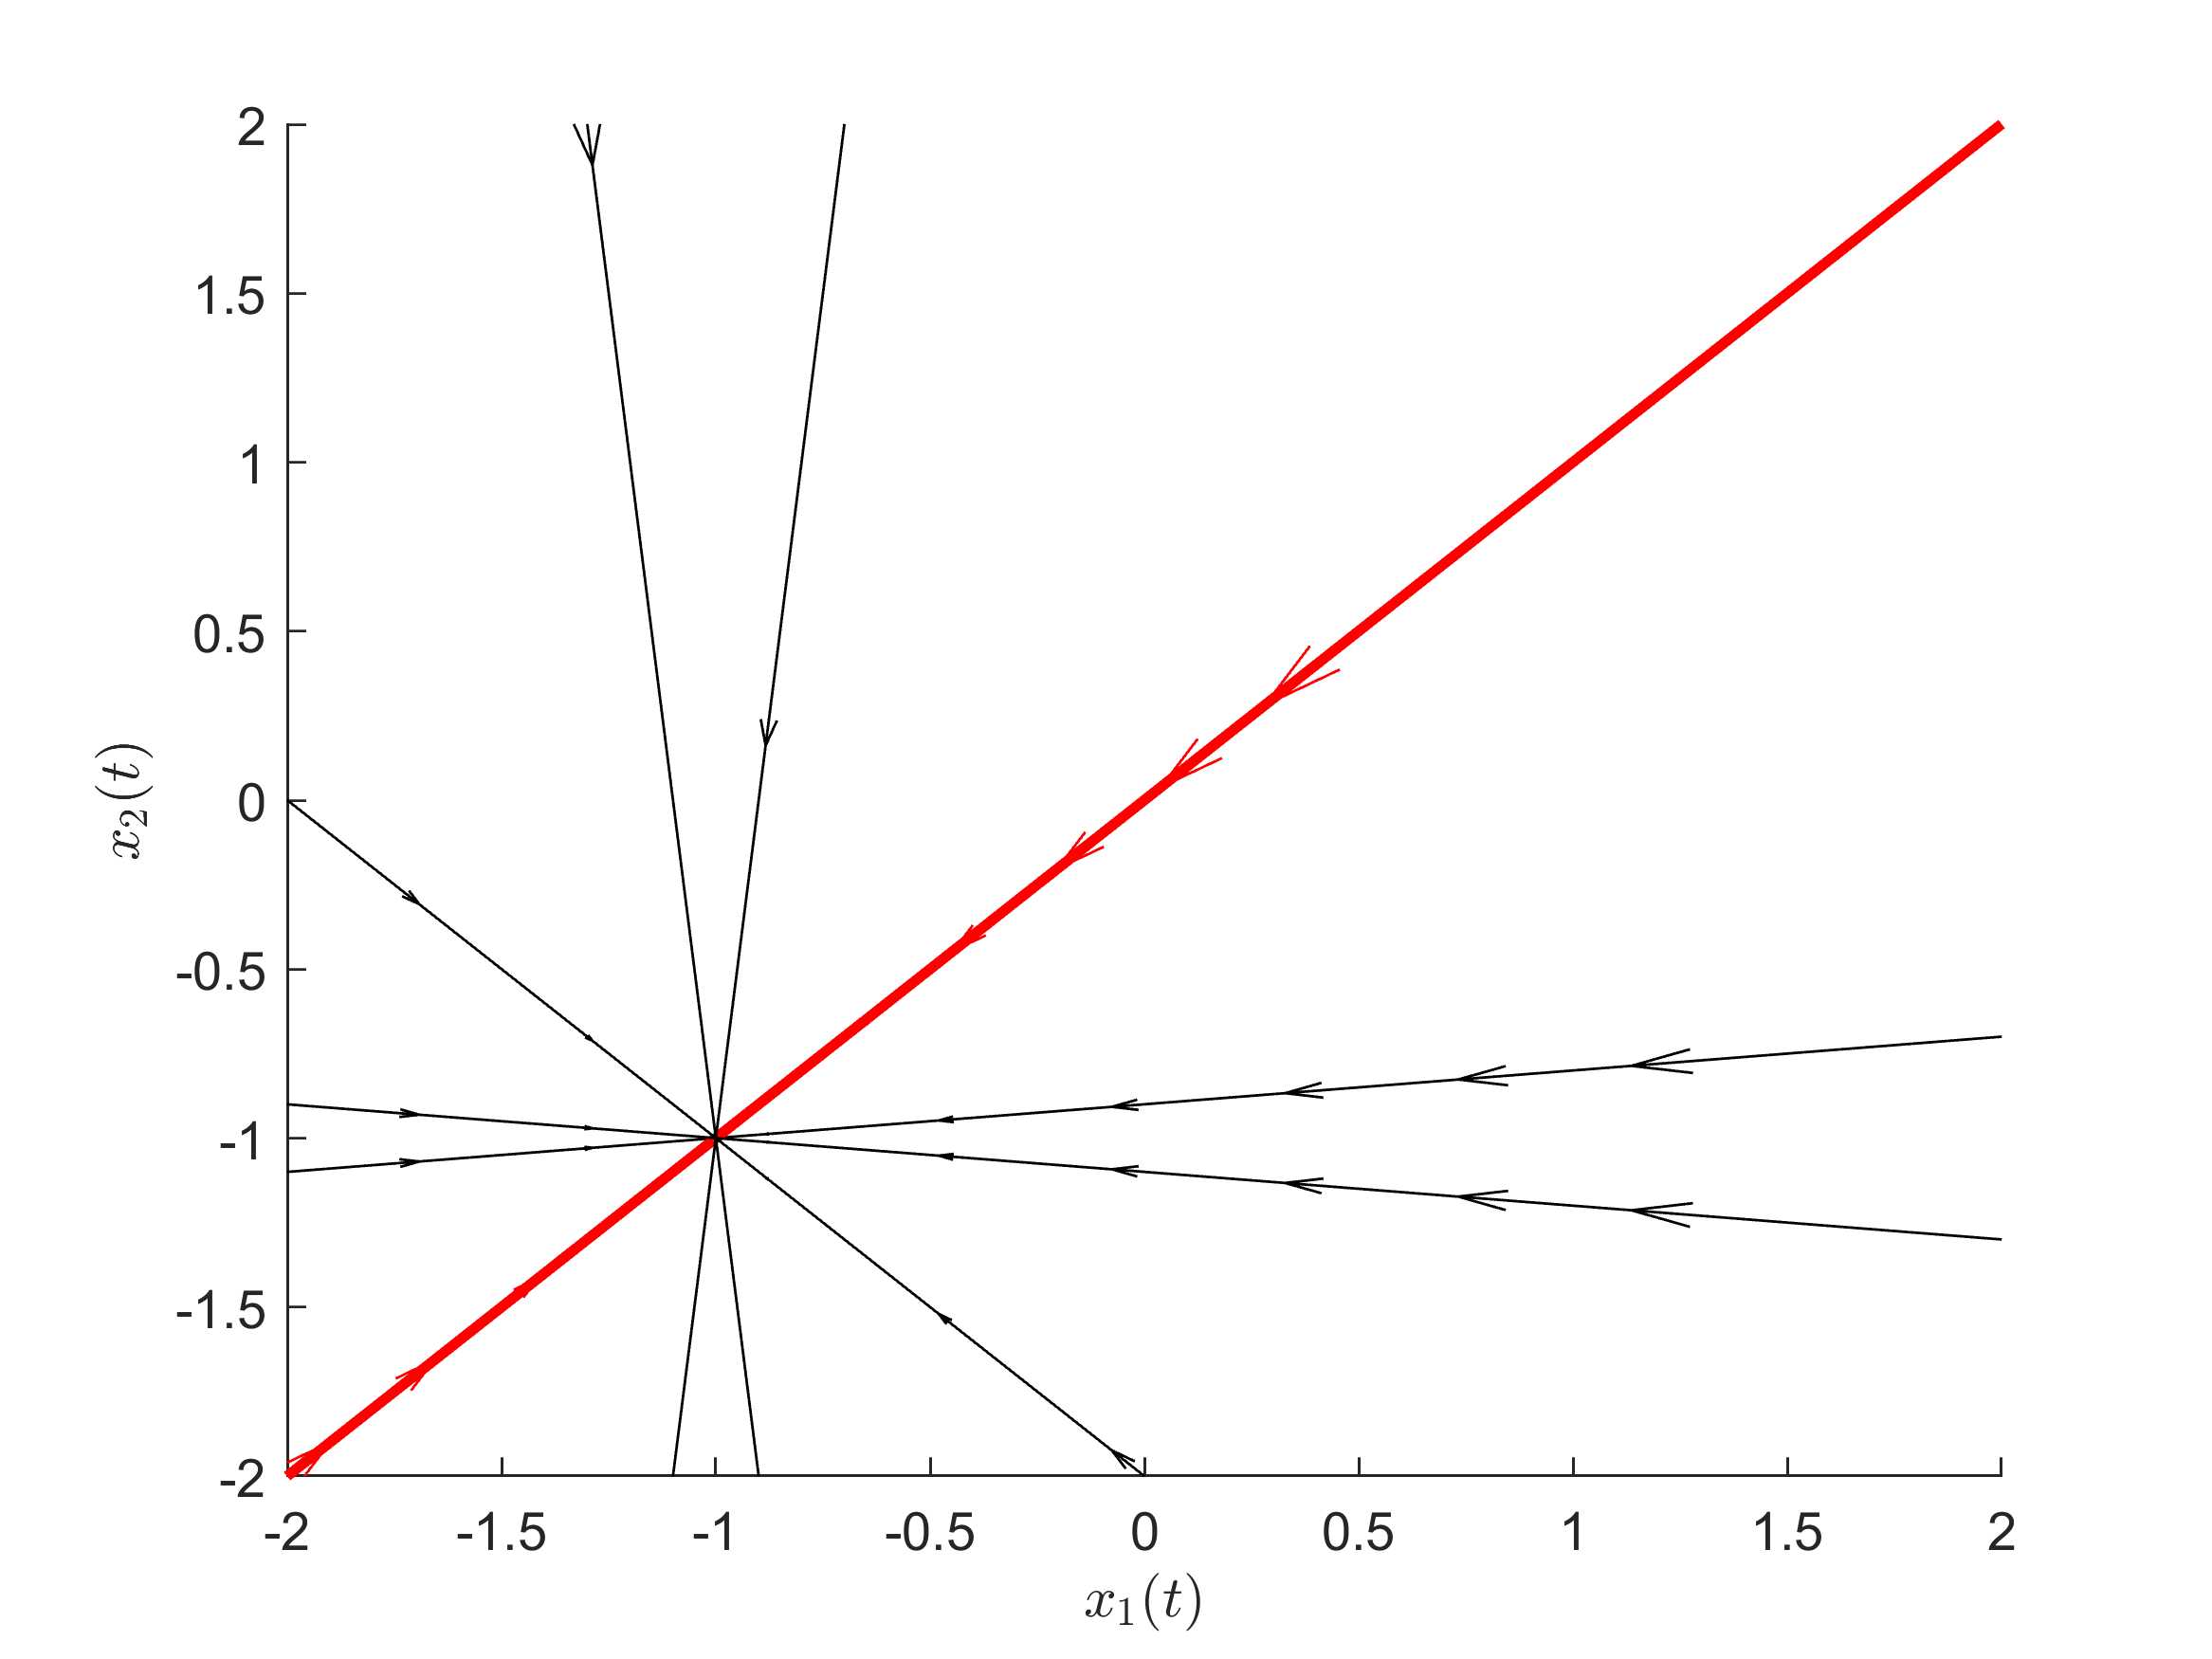
\includegraphics[width=12cm]{../Code/Q4/figures/lowum1x1x2SC.png}
\end{figure}
In figure \ref{x1x2u-1Q4SC} you can see switch curve(red line).
\end{itemize}



